\clearpage


\section{Appendix}\label{sec:appendix}

\begin{figure}[h]
    \begin{align}
        \text{Formula 1:}& \quad i_t = \pi^* + \beta (\pi_t - \pi^*)+\gamma (y_t-\bar{y}) \notag \\[0.5em]
        \text{Formula 2:}& \quad i_t^{SR} = \pi^* + \beta (\pi_t - \pi^*)+\gamma (y_t-\bar{y}) \notag\\[0.5em]
        \text{Formula 3:}& \quad i_t = \pi^* + \phi i_{t-1} + \beta (\pi_t - \pi^*)+\gamma (y_t-\bar{y}) \notag \\[0.5em]
        \text{Formula 4:}& \quad i_t^{SR} = \pi^* + \phi i_{t-1}^{SR} + \beta (\pi_t - \pi^*)+\gamma (y_t-\bar{y}) \notag \\[0.5em] 
        \text{Formula 5:}& \quad i_t = \pi^* + \beta (\mathbb{E}_t[\pi_{t+4}] - \pi^*)+\gamma (y_t-\bar{y}) \notag \\[0.5em]
        \text{Formula 6:}& \quad i_t^{SR} = \pi^* + \beta (\mathbb{E}_t[\pi_{t+4}] - \pi^*)+\gamma (y_t-\bar{y}) \notag\\[0.5em]
        \text{Formula 7:}& \quad i_t = \pi^* + \phi i_{t-1} + \beta (\mathbb{E}_t[\pi_{t+4}] - \pi^*)+\gamma (y_t-\bar{y}) \notag \\[0.5em]
        \text{Formula 8:}& \quad i_t^{SR} = \pi^* + \phi i_{t-1}^{SR} + \beta (\mathbb{E}_t[\pi_{t+4}] - \pi^*)+\gamma (y_t-\bar{y}) \notag
    \end{align}
    \caption{\label{fig:TR_formulas}All Taylor Rule Specifications}
\end{figure}


\begin{figure}[h]
    \centering
    
\includegraphics[width=0.6\textwidth]{figures/raw_data_plot.png}
    \caption[Raw Data Plot]{Plot for our main variables}
    \label{fig:raw_data_plot}
\end{figure}

\begin{figure}[h]
    \centering
    % First Subfigure
    \begin{subfigure}[b]{0.48\textwidth}
        \centering
        
\includegraphics[width=\textwidth]{figures/forecast_plot.png}
        \caption[Forecast Results Plot]{Results for our forecast from 2025 Q4 to 2028 Q1}
        \label{fig:actual_forecast}
    \end{subfigure}
    \hfill % Adds flexible space between the images
    % Second Subfigure
    \begin{subfigure}[b]{0.48\textwidth}
        \centering
        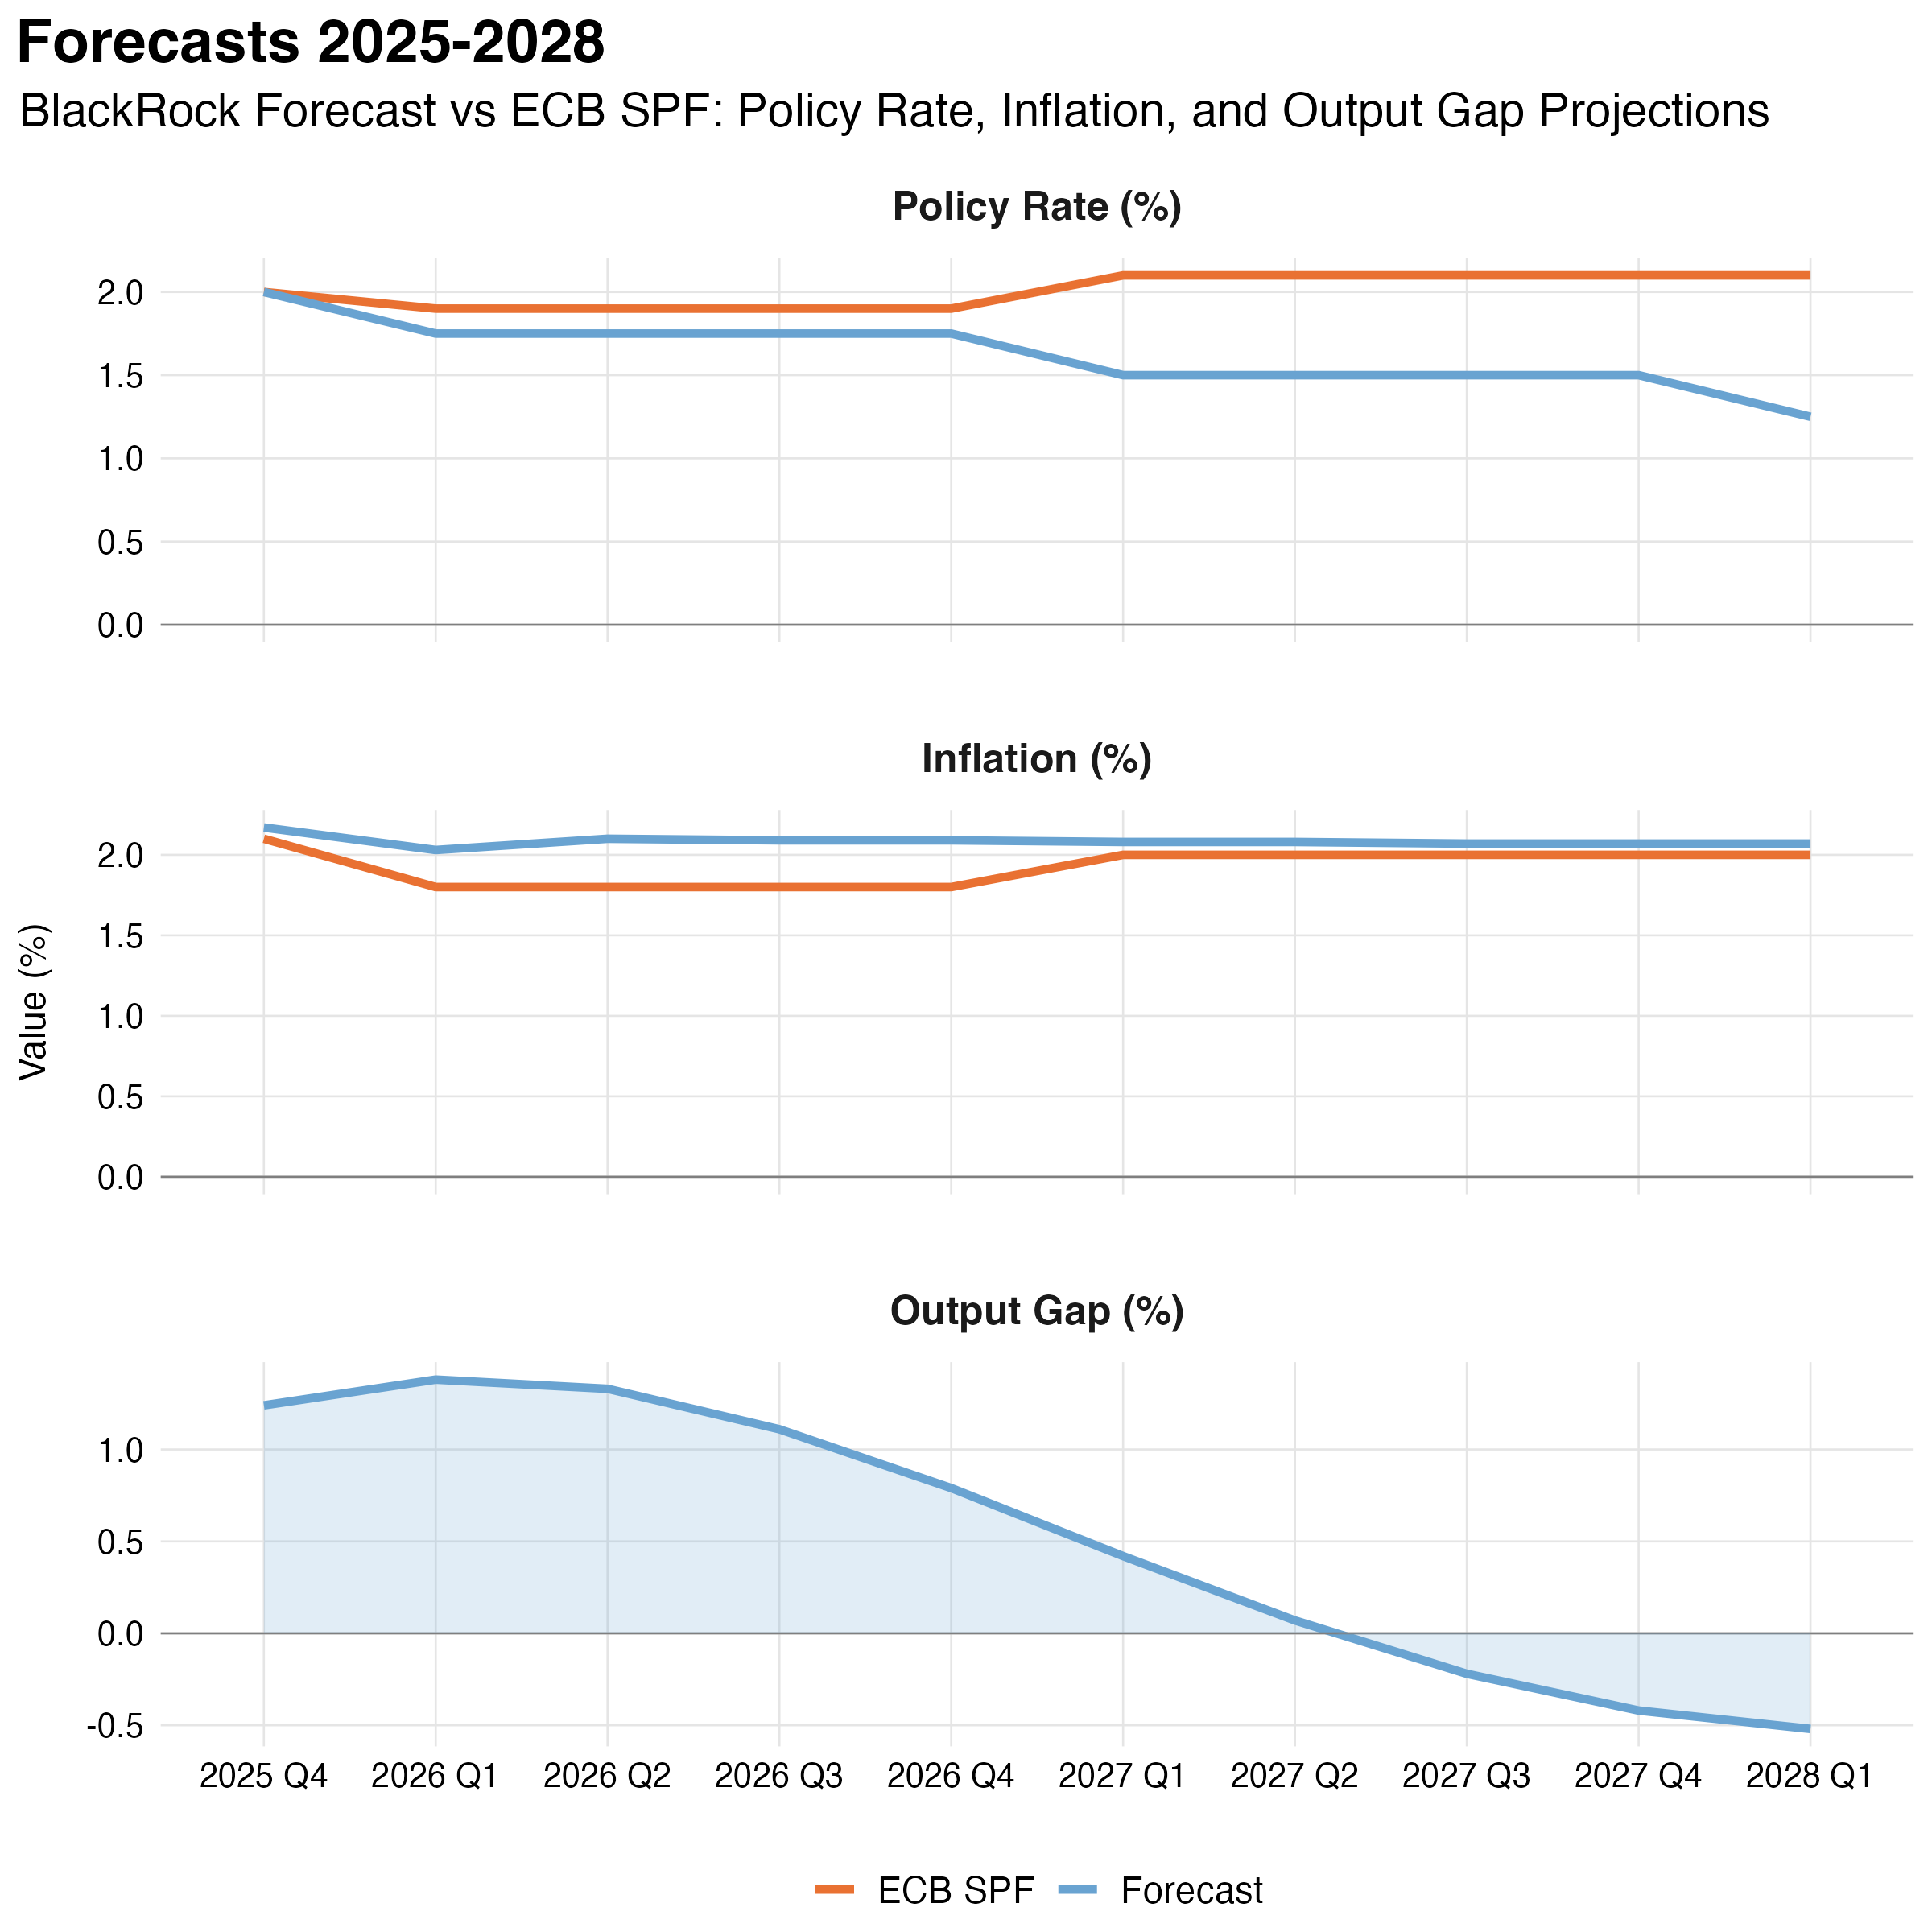
\includegraphics[width=\textwidth]{figures/forecasts_all_comparison.png}
        \caption[Forecast Comparison Plot]{Forecasts Comparison}
        \label{fig:forecast_comparison}
    \end{subfigure}
    \caption{Forecast Results \& Comparison}
    \label{fig:both_forecasts}
\end{figure}

\input{figures/stationarity_results}

\input{figures/Mincer_Zarnowitz_Test_Actual_Rate_with_Lag}

\input{figures/MSFE_Comparison_Trained_on_Actual_Rate_with_Lag}

\begin{figure}[h]
    \centering
    
\includegraphics[width=0.7\textwidth]{figures/spaghetti_errors_plot.png}
    \caption[Forecast Errors Spaghetti Plot]{Spaghetti plot of our forecast errors in evaluation sample, by horizon}
    \label{fig:spaghetti_errors}
\end{figure}

\begin{figure}[h]
    \centering
    % First Subfigure
    \begin{subfigure}[b]{0.48\textwidth}
        \centering
        
\includegraphics[width=\textwidth]{figures/densityridge_plot.png}
        \caption[Forecast Errors Density]{Distribution of our forecast errors}
        \label{fig:errors_density}
    \end{subfigure}
    \hfill % Adds flexible space between the images
    % Second Subfigure
    \begin{subfigure}[b]{0.48\textwidth}
        \centering
        
\includegraphics[width=\textwidth]{figures/FE_var_plot.png}
        \caption[Forecast Errors Variance]{Variance of our forecast errors, by horizon}
        \label{fig:errors_variance}
    \end{subfigure}
    \caption{Properties of Forecast Errors In Evaluation Sample}
    \label{fig:both_errors}
\end{figure}






\begin{comment}
\begin{figure}[h]
    \centering    
    \begin{subfigure}[b]{0.48\textwidth}
        \centering
        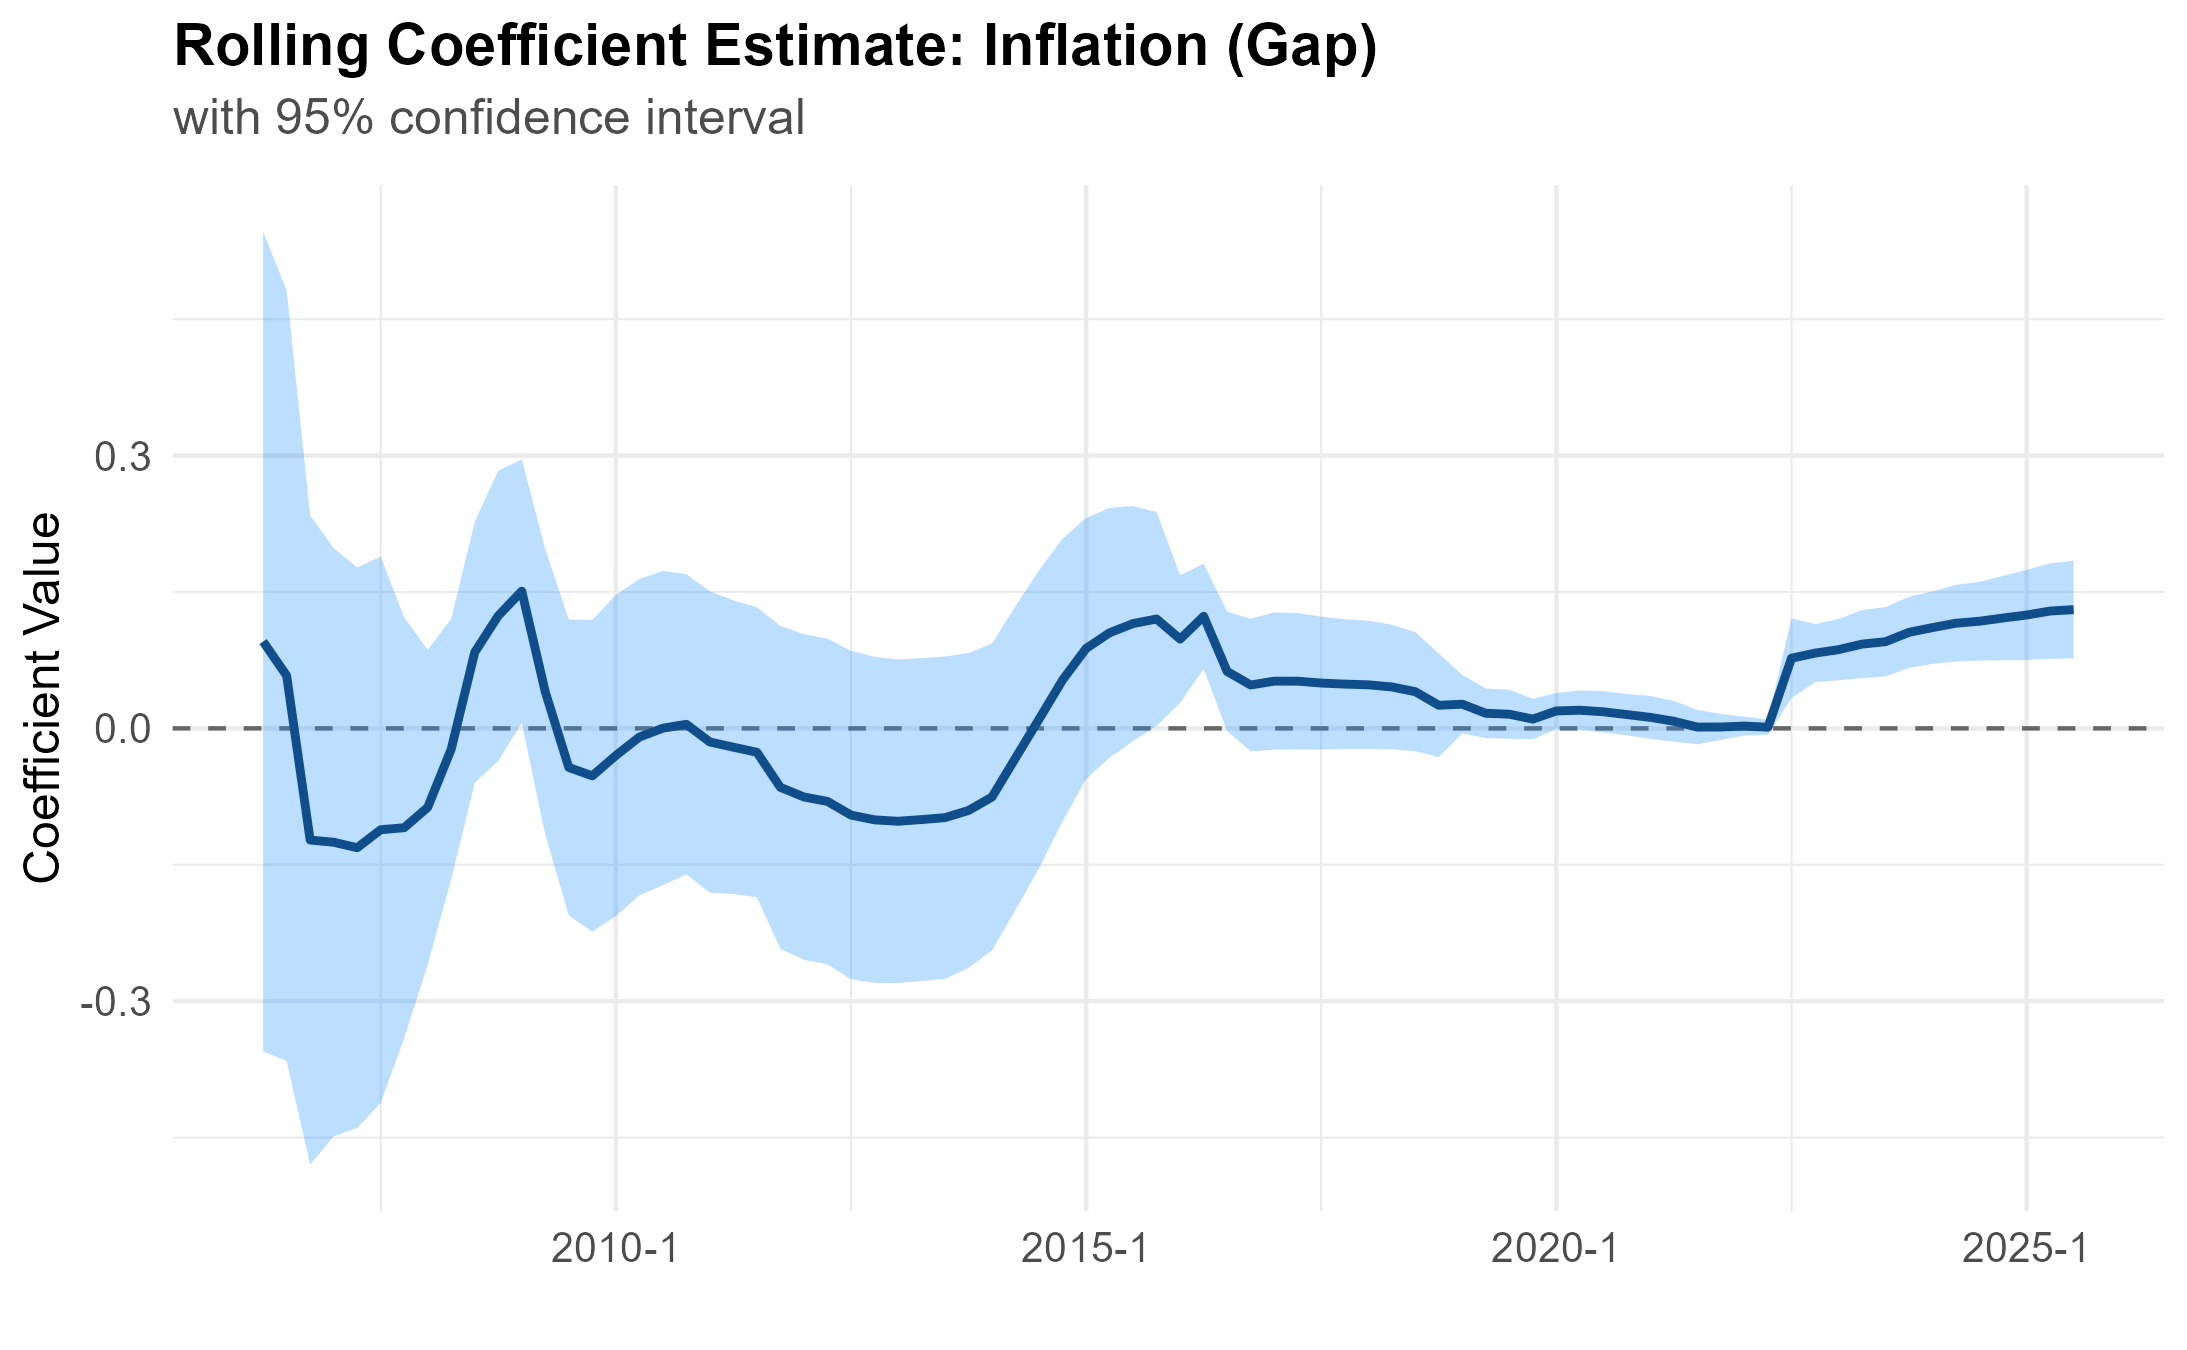
\includegraphics[width=\textwidth]{figures/roll_coef_Inflation (Gap).png}
        %\caption{Inflation Coefficient ($\beta$)}
        \label{fig:roll_TR_inf}
    \end{subfigure}
    \hfill % Adds flexible space between the images
    \begin{subfigure}[b]{0.48\textwidth}
        \centering
        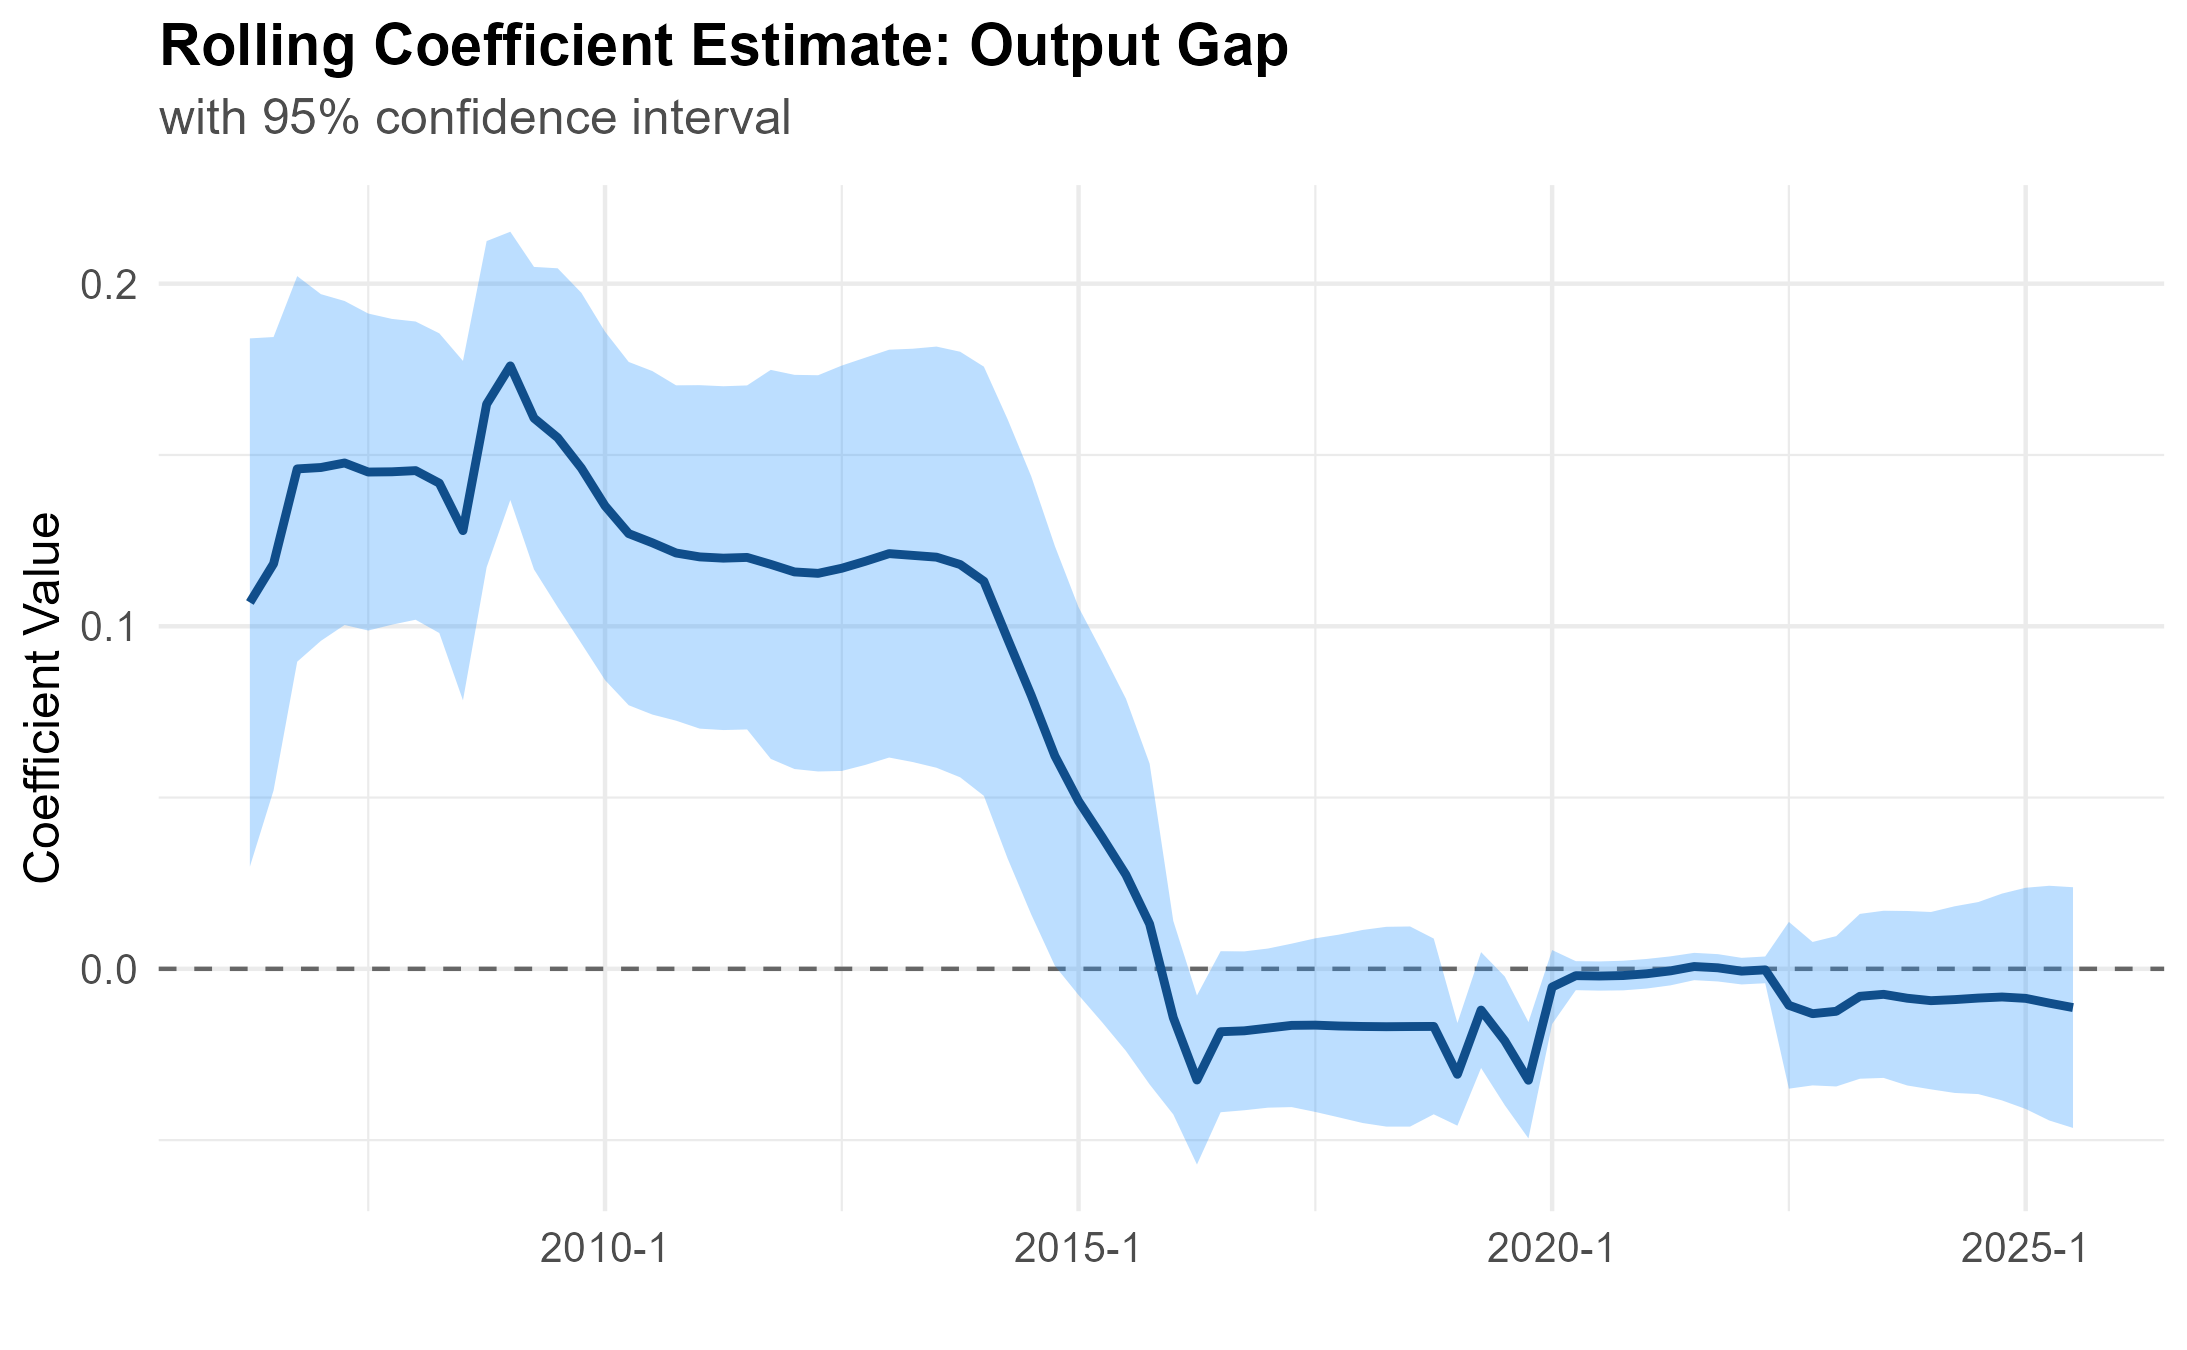
\includegraphics[width=\textwidth]{figures/roll_coef_Output Gap.png}
        %\caption{Output Coefficient ($\gamma$)}
        \label{fig:roll_TR_out}
    \end{subfigure}
    \hfill
    \begin{subfigure}[b]{0.48\textwidth}
        \centering
        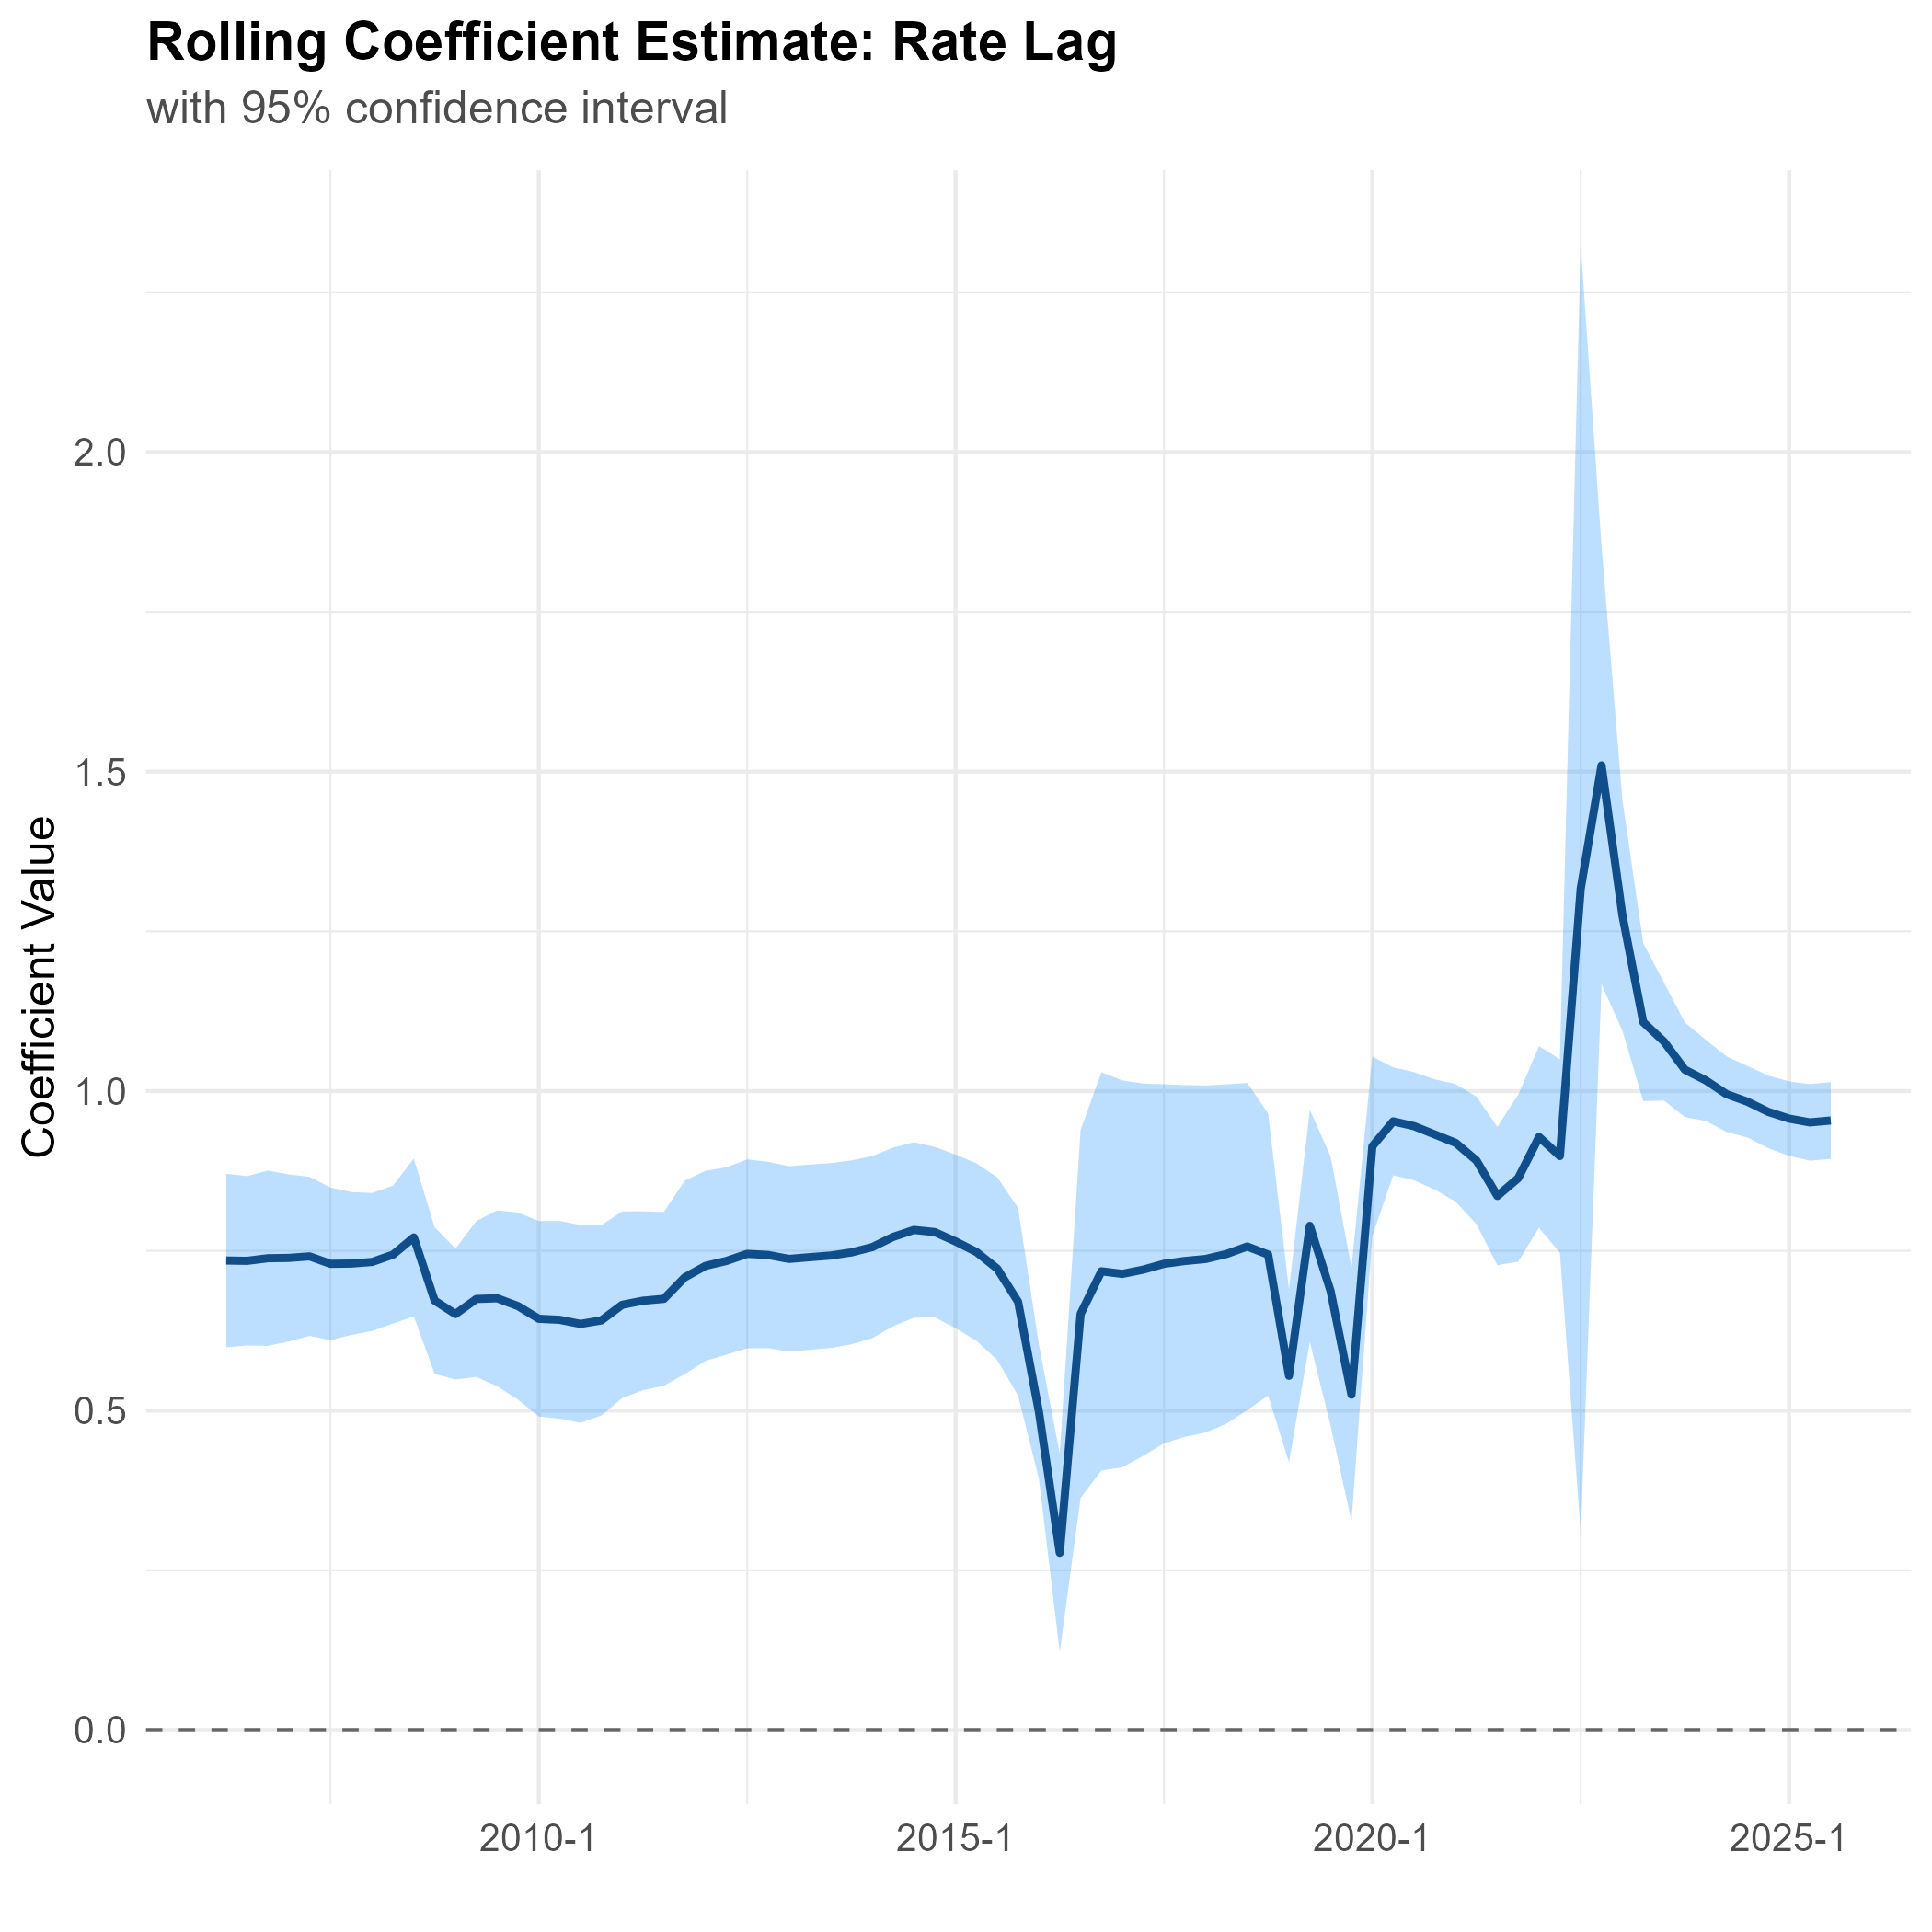
\includegraphics[width=\textwidth]{figures/roll_coef_Rate Lag.png}
        %\caption{Interest Rate Lag Coefficient ($\phi$)}
        \label{fig:roll_TR_lag}
    \end{subfigure}
    \caption{Rolling Taylor Rule Input Coefficients}
    \label{fig:all_TR_coefs}
\end{figure}
\end{comment}

